% Exact LaTeX recreation of the supplied Phase-1.pdf
% Compile with pdfLaTeX. Place member pictures in the same folder if required.

\documentclass[11pt,a4paper]{article}

\usepackage[a4paper,left=2.0cm,right=2.0cm,top=1.55cm,bottom=1.55cm]{geometry}
\usepackage[T1]{fontenc}
\usepackage{lmodern}
\usepackage{graphicx}
\usepackage{xcolor}
\usepackage{array}
\usepackage{tabularx}
\usepackage{ragged2e}
\usepackage{enumitem}
\usepackage{fancyhdr}
\usepackage{tikz}
\usepackage{caption}
\usepackage{setspace}
\usepackage{url}

% -------------------------------------------------
% COLOURS
% -------------------------------------------------
\definecolor{TitleBlue}{RGB}{61,103,154}

% -------------------------------------------------
% GENERAL SETTINGS
% -------------------------------------------------
\setlength{\parindent}{0pt}
\setlength{\parskip}{0pt}
\renewcommand{\arraystretch}{1.0}

% The supplied document uses a clean sans-serif heading style
% and italic serif-style explanatory text.
\newcommand{\blueheading}[1]{%
    {\sffamily\color{TitleBlue}\fontsize{15}{18}\selectfont #1}%
}

\newcommand{\bluebigheading}[1]{%
    {\sffamily\bfseries\color{TitleBlue}\fontsize{16}{19}\selectfont #1}%
}

\newcommand{\instruction}[1]{%
    {\itshape\fontsize{10.5}{12.5}\selectfont #1}%
}

\newcommand{\answerbox}[2][3.0cm]{%
    \vspace{2pt}
    \noindent
    \fbox{%
        \begin{minipage}[t][#1][t]{\dimexpr\textwidth-2\fboxsep-2\fboxrule\relax}
            \vspace{1mm}
            \itshape #2
        \end{minipage}
    }
}

% -------------------------------------------------
% HEADER / FOOTER
% -------------------------------------------------
\pagestyle{fancy}
\fancyhf{}
\renewcommand{\headrulewidth}{0pt}
\renewcommand{\footrulewidth}{0pt}

\fancyhead[L]{%
    \sffamily\bfseries\itshape\fontsize{10.5}{12}\selectfont
    B. TECH CSE | DSCPP-III-2026-T376
}
\fancyhead[R]{%
    \sffamily\bfseries\fontsize{10.5}{12}\selectfont
    PROJECT PROPOSAL
}
\fancyfoot[R]{%
    \itshape\fontsize{10}{12}\selectfont
    Page \thepage
}
\setlength{\headheight}{14pt}
\setlength{\headsep}{23pt}
\setlength{\footskip}{24pt}

% -------------------------------------------------
% PAGE 1
% -------------------------------------------------
\begin{document}

\vspace{8mm}
\bluebigheading{PROJECT AND TEAM INFORMATION}

\vspace{13mm}

\blueheading{Project Title}

\vspace{1mm}

\answerbox[0.8cm]{\begin{center}
{\fontsize{14}{19}\selectfont\textbf{NetMind - Intelligent Network Traffic Analysis and Routing Engine}}
\end{center}}

\vspace{13mm}

\blueheading{Student / Team Information}

\vspace{2mm}

% Team information table
% Compact 4-member layout so all members remain on Page 1.
\noindent
\begin{tabularx}{\textwidth}{|>{\RaggedRight\arraybackslash}p{0.69\textwidth}|>{\RaggedRight\arraybackslash}X|}
\hline
\begin{minipage}[t]{\linewidth}
\vspace{1.5mm}
\textit{Team Name:}\\[-1mm]
\textit{Team \#}
\vspace{1.5mm}
\end{minipage}
&
\begin{minipage}[t]{\linewidth}
\vspace{1.5mm}
\textit{CodeGraphers}
\\
\textit{DSCPP-III-2026-T376}
\vspace{1.5mm}
\end{minipage}
\\
\hline
\begin{minipage}[t][3.25cm][t]{\linewidth}
\vspace{1.5mm}
\textbf{Team member 1 (Team Lead)}\\[-1mm]
\textit{(Last Name, name: student ID: email, picture):}
\vspace{2.0cm}
\end{minipage}
&
\begin{minipage}[t][3.25cm][t]{\linewidth}
\vspace{1.5mm}
\textit{Garg, Shristy -- 2028154}\\
\textit{2510280123@geu.ac.in}

\vspace{2mm}
\includegraphics[width=3.0cm,height=1.5cm,keepaspectratio]{member1.jpeg}
\end{minipage}
\\
\hline
\begin{minipage}[t][3.25cm][t]{\linewidth}
\vspace{1.5mm}
\textbf{Team member 2}\\[-1mm]
\textit{(Last Name, name: student ID: email, picture):}
\vspace{2.0cm}
\end{minipage}
&
\begin{minipage}[t][3.25cm][t]{\linewidth}
\vspace{1.5mm}
\textit{Ojha, Gungun -- 2027788}\\
\textit{2510012505@geu.ac.in}

\vspace{2mm}
\includegraphics[width=3.0cm,height=1.5cm,keepaspectratio]{member2.jpeg}
\end{minipage}
\\
\hline
\begin{minipage}[t][3.25cm][t]{\linewidth}
\vspace{1.5mm}
\textbf{Team member 3}\\[-1mm]
\textit{(Last Name, name: student ID: email, picture):}
\vspace{2.0cm}
\end{minipage}
&
\begin{minipage}[t][3.25cm][t]{\linewidth}
\vspace{1.5mm}
\textit{Mittra, Shrijit -- 2028854}\\
\textit{2510370385@geu.ac.in}

\vspace{2mm}
\includegraphics[width=3.0cm,height=1.5cm,keepaspectratio]{member3.jpeg}
\end{minipage}
\\
\hline

\end{tabularx}

\vspace{3mm}

\begin{minipage}[t][3.25cm][t]{\linewidth}
\vspace{1.5mm}
\textbf{Mentor: }
\textit{Dr. Vidit Kumar}
\\
\textbf{Email: }
\textit{viditkumar.cse@geu.ac.in}
\end{minipage}

\newpage

% -------------------------------------------------
% PAGE 2
% -------------------------------------------------

\bluebigheading{PROPOSAL DESCRIPTION (10 pts)}

\vspace{10mm}

\blueheading{Motivation (1 pt)}

\vspace{1mm}

\answerbox[11.0cm]{Computer networks nowadays generate large amount of traffic that need to be continuously monitored, analysed, and routed efficiently. Traditional network monitoring and simulation software provides insightful metrics such as latency, bandwidth utilisation, throughput, packet loss, jitter and congestion. These tools however primarily focus on monitoring and visualisation and the user finds it difficult to experiment with the relationship between network topology, traffic behaviour, routing algorithms, and changing network conditions in one integrated environment.

The motivation for NetMind is to create an educational yet technically substantial platform, combining network modeling, traffic simulation, graph based routing, standardised network metrics, and intelligent analysis. Routers, hosts and communication links are represented as a dynamic graph, allowing different network topologies and traffic conditions to be simulated and studied.

Unlike conventional monitoring tools, which primarily report what is happening, NetMind's primary focus is to help users understand why a network behaviour occurs and how different routing strategies respond to it. Algorithms such as Breadth-first search, Depth-first search, Djikstra's algorithm, and other routing approaches can be implemented, compared, and evaluated using measurable network performance metrics.

Limitations of the approach of pure rule-based analysis are also discussed in NetMind. NetMind uses machine learning for performing operations like analyzing traffic patterns, detecting anomalies, and forecasting network status. The GraphRAG feature links network topology, past observations, metrics, and events together to provide context-aware explanations and querying.

NetMind brings OOP, data structures, graph algorithms, computer networking, simulation, machine learning, and knowledge retrieval together in a single system, providing both practical experimentation and deeper insight into network behavior.}

\vspace{7mm}

\blueheading{State of the Art / Current solution (1 pt)}

\vspace{1mm}

\answerbox[7.65cm]{Monitoring and analysing networks are done using specialized software that is used for different features of the networks. For instance, Wireshark is a software used for packet capture and protocol analysis. On the other hand, performance monitoring of a network is achieved by software such as SolarWinds Network Performance Monitor which captures latency, packet loss, bandwidth utilization, throughput, availability, and device health. It also allows automatic discovery of the devices within the network, along with visualising network topologies and analysing traffic flows.

Network simulation and troubleshooting tools provide another approach. For example, Cisco's packet-tracer functionality can simulate packet flows and trace their paths through routing and security policies.

However, these capabilities are generally distributed across specialised tools, with their internal routing algorithms and analytical processes largely abstracted from users. NetMind proposes an integrated, educational platform combining graph-based network modeling, traffic simulation, standard network performance metrics, classical routing algorithms, ML-based traffic intelligence, and knowledge-aware analysis. This enables users not only to monitor network behaviour, but also to experiment with and understand the algorithms and decisions responsible for that behaviour.}

\vspace{30mm}

\blueheading{Project Goals and Milestones (2 pts)}

\vspace{1mm}

\answerbox[16cm]{Project goals:\newline The primary goal of NetMind is to develop an engine for network traffic analysis, simulation and routing based on graphs. The system aims to model a network infrastructure, simulate a realistic traffic environment, measure standard performance metrics for the network, and evaluate different routing strategies under changing network conditions.
\newline
The project specifically aims to:

1. Design an object oriented model for hosts, routers, links, packets, flows, and network events.
2. Model the network topology using graphs and implement fundamental graph and routing algorithms.
3. Simulate network traffic, congestion, failures, and changing link conditions.
4. Measure standard metrics such as throughput, latency, jitter, packet loss, bandwidth utilization, hop count, and network reliability.
5. Evaluate the performance of various routing algorithms in different network conditions.
6. Implement machine learning to analyse traffic patterns, detect anomalies, and predict network conditions.
7. Integrate GraphRAG to perform context-aware querying and interpretation of network topology, metrics, events, and historical observations.
8. Provide a clear visualisation and analysis interface for understanding network behaviour and algorithmic decisions.\newline \newline
Milestones:\newline
Milestone 1 — System Foundation: Define architecture, project structure, core classes, enumerations, and build system.

Milestone 2 — Network and Graph Engine: Implement network entities, graph representation, topology management, traversal algorithms, and graph metrics.

Milestone 3 — Traffic Simulation and Metrics: Implement packet/flow simulation, network events, congestion/failure scenarios, and standard networking metrics.

Milestone 4 — Routing Engine: Implement and compare multiple routing algorithms under simulated network conditions.

Milestone 5 — ML Intelligence: Prepare datasets from simulations and integrate ML-based traffic analysis, anomaly detection, and network-condition prediction.

Milestone 6 — GraphRAG and Knowledge Layer: Build a knowledge representation of network topology, metrics, events, and historical results for natural-language, context-aware analysis.

Milestone 7 — Integration and Evaluation: Integrate all components, develop visualization, conduct experiments, compare results, optimize performance, and prepare the final demonstration and documentation.}

\vspace{100mm}

\blueheading{Project Approach (3 pts)}

\vspace{1mm}

\answerbox[10cm]{NetMind would be a modular, layered system, combining computer network, OOP, data structures and algorithms, simulation, machine learning, and graph-based knowledge retrieval.

The network engine will be programmed using C++ through an object-oriented approach. The objects such as Routers, hosts, links, packets, flows, and network events will be modeled using different classes. The network topology will be handled using graph data structures. Appropriate data structures like adjacency list, priority queues, hash maps, and queues will be used in the algorithms.

The traffic simulation engine will generate and process the packets and traffic-flow events, while dynamically changing the network conditions conditions such as bandwidth, latency, congestion, packet loss, and link failures. Standard network metrics will be collected at link, host, router, and network levels. Routing algorithms will then be evaluated using these metrics under identical simulated scenarios.

Python, together with relevant libraries like Pandas, NumPy, Scikit-learn and Matplotlib will be employed for the ML and data-analysis layer. Datasets for analysis of traffic patterns, detection of anomalies and predicting network conditions will be compiled based on the results of the C++ engine simulations.

A GraphRAG-based knowledge layer will connect network topology, metrics, events, routing decisions, and historical observations, allowing users to query the simulated network and obtain context-aware explanations.

The final system will provide a visualization/dashboard layer to display topology, traffic, metrics, routing paths, failures, and analytical results.
}

\newpage

% -------------------------------------------------
% PAGE 3
% -------------------------------------------------

\blueheading{System Architecture (High Level Diagram)(2 pts)}

\vspace{3mm}

\begin{center}

\begin{tikzpicture}[
    box/.style={
        rectangle,
        draw=TitleBlue,
        thick,
        rounded corners=3pt,
        align=center,
        minimum width=38mm,
        minimum height=11mm,
        font=\itshape\fontsize{10.5}{12.5}\selectfont
    },
    arrow/.style={
        ->,
        thick
    },
    dashedarrow/.style={
        ->,
        thick,
        dashed
    }
]

\node[box] (user) at (-2.5,0)
    {User / Network Analyst};

\node[box] (interface) at (2.5,0)
    {Visualization \&\\Interactive Interface};


\node[box] (controller) at (0,-2)
    {Application Controller\\\& Scenario Manager};


\node[box] (network) at (-4,-4.2)
    {Network Model\\
     \scriptsize Routers, Hosts, Links, Packets};

\node[box] (graph) at (4,-4.2)
    {Graph \& DSA Engine\\
     \scriptsize BFS, DFS, Graph Structures};


\node[box] (routing) at (-4,-6.5)
    {Routing Engine\\
     \scriptsize Dijkstra \& Alternative Algorithms};

\node[box] (simulation) at (4,-6.5)
    {Traffic Simulation Engine\\
     \scriptsize Traffic, Queues, Congestion, Failures};


\node[box] (metrics) at (0,-8.8)
    {Network Metrics \& Analytics\\
     \scriptsize Throughput, Latency, Jitter, Loss, Utilization};


\node[box] (storage) at (0,-11.2)
    {Data \& Experiment Storage\\
     \scriptsize Metrics, Traffic, Events, Topology, History};


\node[box] (ml) at (-4,-14.2)
    {Machine Learning\\
     \scriptsize Traffic Patterns, Anomaly Detection, Prediction};

\node[box] (rag) at (4,-14.2)
    {GraphRAG / Knowledge Layer\\
     \scriptsize Knowledge Graph, Retrieval, Explanations};


\draw[arrow] (user) -- (interface);
\draw[arrow] (interface) -- (user);

\draw[arrow] (interface) -- (controller);
\draw[arrow] (controller) -- (interface);


\draw[arrow] (controller) -- (network);
\draw[arrow] (controller) -- (graph);


\draw[arrow] (network) -- (routing);
\draw[arrow] (graph) -- (routing);

\draw[arrow] (network) -- (simulation);
\draw[arrow] (routing) -- (simulation);
\draw[arrow] (graph) -- (simulation);


\draw[arrow] (routing) -- (metrics);
\draw[arrow] (simulation) -- (metrics);


\draw[arrow] (metrics) -- (storage);


\draw[arrow] (storage) -- (ml);
\draw[arrow] (storage) -- (rag);


\draw[arrow]
    (ml.west)
    -- (-8,-14.2)
    -- (-8,-2)
    -- (controller.west);

\draw[arrow]
    (rag.east)
    -- (8,-14.2)
    -- (8,-2)
    -- (controller.east);

\end{tikzpicture}

\end{center}

\begin{center}
\small
\textit{Figure: High-Level System Architecture of NetMind}
\end{center}

\vspace{300mm}

\blueheading{Project Outcome / Deliverables (1 pts)}

\vspace{1mm}

\answerbox[11cm]{The primary outcome of this project would be a functional prototype of NetMind, which would an intelligent system for analysis of network traffic, simulation and routing on the network. It would integrate both classical networking algorithms and data-driven analysis.
\newline \newline
The major deliverables will include:

1. Network Modeling and Graph Engine: An object-oriented C++ implementation for representing routers, hosts, links, packets, traffic flows, and network topology using appropriate graph and data structures.\newline
2. Traffic Simulation Engine: A simulation environment capable of generating network traffic and modeling congestion, changing link conditions, packet loss, latency, and network failures.\newline
3. Routing Engine: Implementation of multiple routing algorithms, including Dijkstra and alternative routing strategies, with comparative evaluation based on network conditions and performance metrics.\newline
4. Network Metrics and Analytics: Measurement and visualization of standard metrics including throughput, latency, RTT, jitter, packet loss, bandwidth utilization, hop count, and reliability.\newline
5. Machine Learning Module: Python-based models for traffic pattern analysis, anomaly detection, and prediction of relevant network conditions using datasets generated from simulations.\newline
6. GraphRAG Knowledge Layer: A knowledge and retrieval system connecting topology, traffic, metrics, events, routing decisions, and historical experiments to provide context-aware network analysis and explanations.\newline
7. Visualization and Documentation: An interactive interface for viewing topology, traffic behavior, routing paths, metrics, detected anomalies, and experiment results, along with technical documentation, test results, and comparative performance analysis.}

\vspace{7mm}

\blueheading{Assumptions}

\vspace{1mm}

\answerbox[4cm]{The project assumes a simulated network environment in which routers, hosts, links, and traffic flows can be represented using simplified but realistic network parameters. Link properties such as bandwidth, latency, packet loss, and reliability are assumed to remain constant or change according to predefined simulation events. Routing algorithms are evaluated using identical network scenarios to ensure fair comparison. The ML models are assumed to be trained on sufficiently representative datasets generated from simulations. GraphRAG is assumed to operate on structured network knowledge, historical experiments, metrics, and events. The system focuses on simulation and analysis rather than controlling or modifying real-world network infrastructure.}

\vspace{7mm}

\blueheading{References}

\vspace{1mm}

\answerbox[6cm]{

> Harvard CS145 — Routing Network Simulator\newline
\url{https://github.com/Harvard-CS145/routing}

> NetSimCPP — C++ Network Simulator\newline
\url{https://github.com/UmarlyPoeta/inzynieria_oprogramowania}

> Wireshark — Network Protocol Analyzer and Packet Analysis Resources\newline
\url{https://www.wireshark.org/}

> Microsoft GraphRAG\newline
\url{https://github.com/microsoft/graphrag}

> Flow simulator -- C++\newline
\url{https://github.com/jianglong-nie/Flow-Simulator}

> From statistical- to machine learning-based network traffic prediction\newline
\url{https://onlinelibrary.wiley.com/doi/10.1002/ett.4394}

}
\end{document}
